\documentclass[../../main.tex]{subfiles}
\begin{document}
\chapter{Pose Matching for Low Level Synthesis}
\label{ch:pose_matching}


todo, fix/polish
In the previous chapters, we looked at granularity in sign language animation based on AZee's structure. However, one of the key missing pieces in our study was the ability to shortcut or match a posture state on generated low level poses. todo, moe intro posematching

The past decade has seen a rise in deep learning technologies in in the field of character animation. These technologies have been used to generate realistic and expressive animations for a wide range of applications, from video games to virtual reality. One of the key challenges in character animation is the generation of natural and fluid motion, which requires the ability to capture the nuances of human movement and behavior. 

Motion matching is a technique that aims to address this challenge by matching the motion of a character to a set of predefined poses or movements. By comparing the motion of the character to a database of motion data, motion matching can generate more realistic and contextually appropriate animations.

The use of avatars for sign language generation offers several advantages. Avatars can be programmed to perform a wide range of gestures with high precision, and they provide a consistent visual representation that can be customized to match the user's preferences. Moreover, avatars can be deployed in various digital environments, such as websites, mobile applications, and virtual reality platforms, making them a versatile tool for improving accessibility.

In this work, we focus on the development of a motion generation system for sign language using a pose prior model derived from a sign language dataset. The pose prior model captures the typical poses and movements associated with different signs, providing a statistical framework that guides the motion generation process. By learning these priors from a large dataset, our system is able to generate realistic and contextually appropriate sign language gestures in real time.

Our approach builds on the foundation of existing research in avatar-based sign language generation while introducing several key innovations. First, we employed a data-driven method to learn the pose priors, using a deep learning model trained on a diverse sign language dataset. This contrasts with earlier methods that relied on manually crafted animations or rule-based systems, which often lacked flexibility and struggled to generalize to new signs or contexts.

Second, we incorporated temporal dynamics into our motion generation model, recognizing that sign language gestures are inherently dynamic and involve continuous motion. This was achieved by extending the pose prior model to account for the temporal evolution of gestures, enabling the avatar to generate fluid and natural movements that accurately reflect the timing and flow of real sign language.

Third, we evaluated the performance of our avatar-based motion generation system in various scenarios, including real-time applications where the avatar must respond quickly to changing inputs. Our experiments demonstrated that the use of pose priors significantly improves the quality and accuracy of the generated gestures, making the system suitable for a wide range of applications, from sign language translation services to educational tools for sign language learners.

The potential impact of avatar-based sign language generation is substantial. By providing a means for generating sign language in real-time, these systems can facilitate communication between Deaf and hearing individuals, support language learning, and enhance the accessibility of digital content. Furthermore, the techniques developed in this work can be extended to other areas of motion generation, such as gesture-based control systems and virtual character animation.

However, despite these advancements, challenges remain. One of the primary challenges is the diversity of sign languages and the need to create models that can accommodate different sign languages, each with its own grammar, lexicon, and cultural nuances. Additionally, the variability in individual signing styles introduces further complexity, as the system must be able to adapt to different users. Addressing these challenges will require ongoing research and collaboration between technologists, linguists, and the Deaf community.

In summary, this chapter presents our approach to sign language motion generation using an avatar-based system driven by pose priors learned from a sign language dataset. We discuss the theoretical foundations of our method, the practical considerations in its implementation, and the results of our experimental evaluations. Through this work, we aim to contribute to the ongoing efforts to create more accessible and inclusive technologies that bridge the communication gap between the Deaf and hearing worlds.


In this chapter, we take a step in this direction by leveraging the low level synthesis techniques we looked in Chapter \ref{ch:multi_track} to create a motion matching system which is capable to generate more natural poses.
The chapter is structured as follows. In Section \ref{sec:todo}, we .... In Section \ref{sec:todo}, we .... Next, in Section \ref{sec:todo}, .... In Section \ref{sec:todo}, .... Finally, in Section \ref{sec:todo}, we conclude the chapter with our final remarks.

\section{Related work}
\label{sec:related_work}

In this section, we discuss relevant background work in pose matching, focusing on classical methods, data-driven approaches, and the integration of latent space representations. These methodologies form the foundation for understanding advancements in character animation.

\subsection{Classical Inverse Kinematics (IK) Methods}
\label{subsec:classical_ik}

Classical Inverse Kinematics (IK) methods have been a cornerstone in the field of character animation, providing techniques to determine the necessary joint angles to achieve a desired end-effector position. Some of these methods are Jacobian-based approach \cite{TODO itasc}, Cyclic Coordinate Descent (CCD)\cite{TODO}, and Forward And Backward Reaching Inverse Kinematics (FABRIK)\cite{TODO}.

Jacobian-Based Methods involve computing the Jacobian matrix to linearize the relationship between joint angles and end-effector positions. By iteratively adjusting joint angles to reduce the error between the current and target positions, these methods offer a robust solution for real-time applications\ref{fig:jacobian_based}. However, they often require complex matrix operations and are sensitive to singularities, making them less suitable for more complex animations [TODO].

\begin{figure}
    \centering 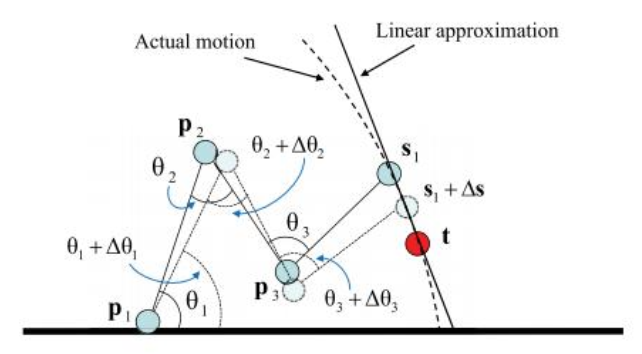
\includegraphics[width = 2.5in]{chapters/pose_matching/images/jacobian_based.png}
    \caption{Jacobian based(iTasC) IK solving}
    \label{fig:jacobian_based}
\end{figure}

Cyclic Coordinate Descent (CCD) simplifies the IK problem by iteratively adjusting one joint at a time, minimizing the distance between the end-effector and the target\ref{fig:ccdik}. CCD is computationally efficient and easy to implement, making it popular in game engines. However, its greedy approach can lead to suboptimal solutions, especially in highly constrained scenarios\cite{TODO}.

\begin{figure}
  \centering 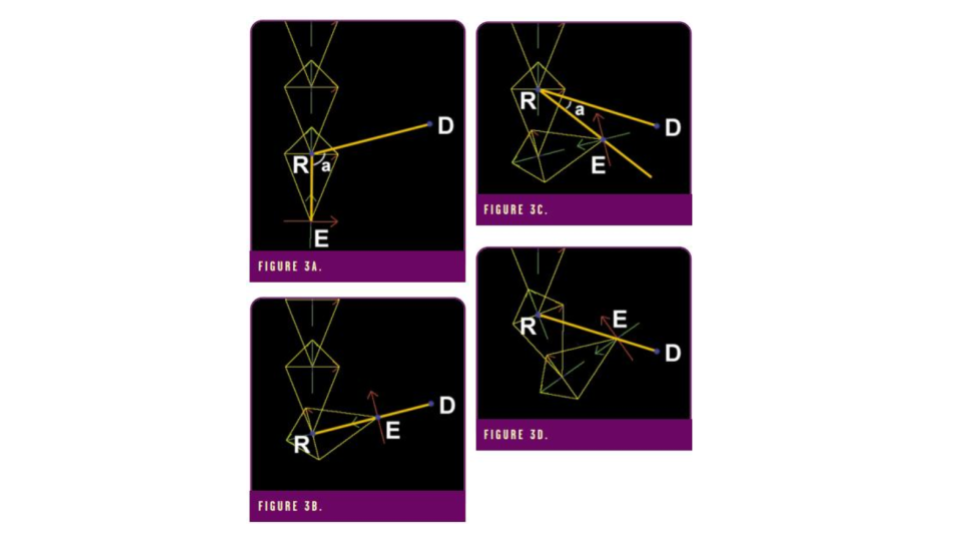
\includegraphics[width = 2.5in]{chapters/pose_matching/images/ccdik.png}
  \caption{Cyclic Coordinate Descent (CCD) IK solving}
  \label{fig:ccdik}
\end{figure}

FABRIK differs from other methods by focusing on the positions of joints rather than their angles. It iteratively adjusts the positions of joints through a two-pass approach, first from the end-effector to the root and then from the root to the end-effector\ref{fig:fabrik}. This method is known for its simplicity and stability, particularly in scenarios where maintaining a natural joint configuration is crucial\cite{TODO}.

\begin{figure}
  \centering 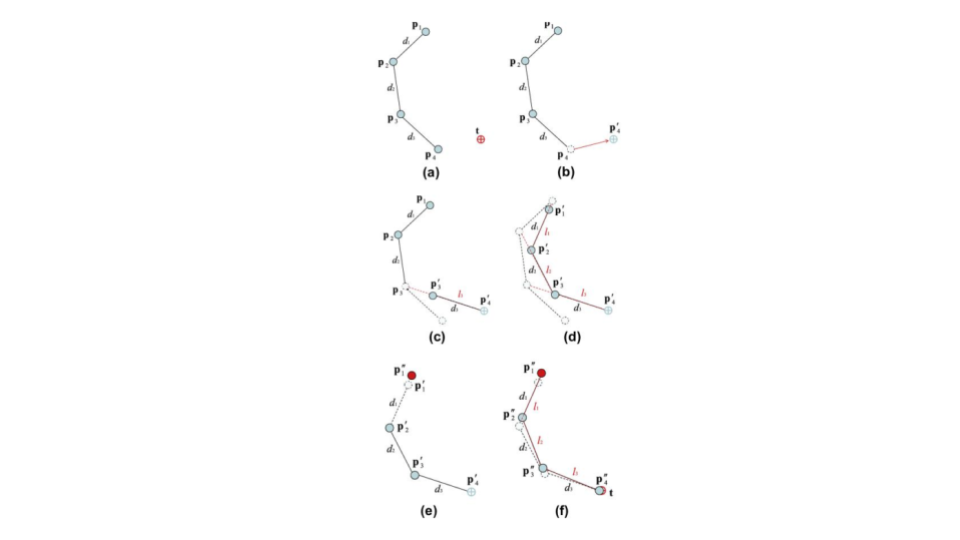
\includegraphics[width = 2.5in]{chapters/pose_matching/images/fabrik.png}
  \caption{Forward And Backward Reaching Inverse Kinematics(FABRIK) solving}
  \label{fig:fabrik}
\end{figure}

These classical methods have been widely adopted due to their balance between computational efficiency and control, making them suitable for a variety of real-time applications. However, they have notable limitations. They are prone to singularities, where solutions become unstable, and often require significant computational resources, especially in complex or high-dimensional systems. The resulting movements can sometimes be unnatural or biomechanically unrealistic, particularly when handling joint limits or multiple end-effectors. Additionally, these methods struggle with complex constraints and often produce suboptimal solutions that may not adapt well to varying scenarios, making them less suitable for dynamic or highly detailed applications \ref{fig:problems_classical}.

\begin{figure}
  \centering 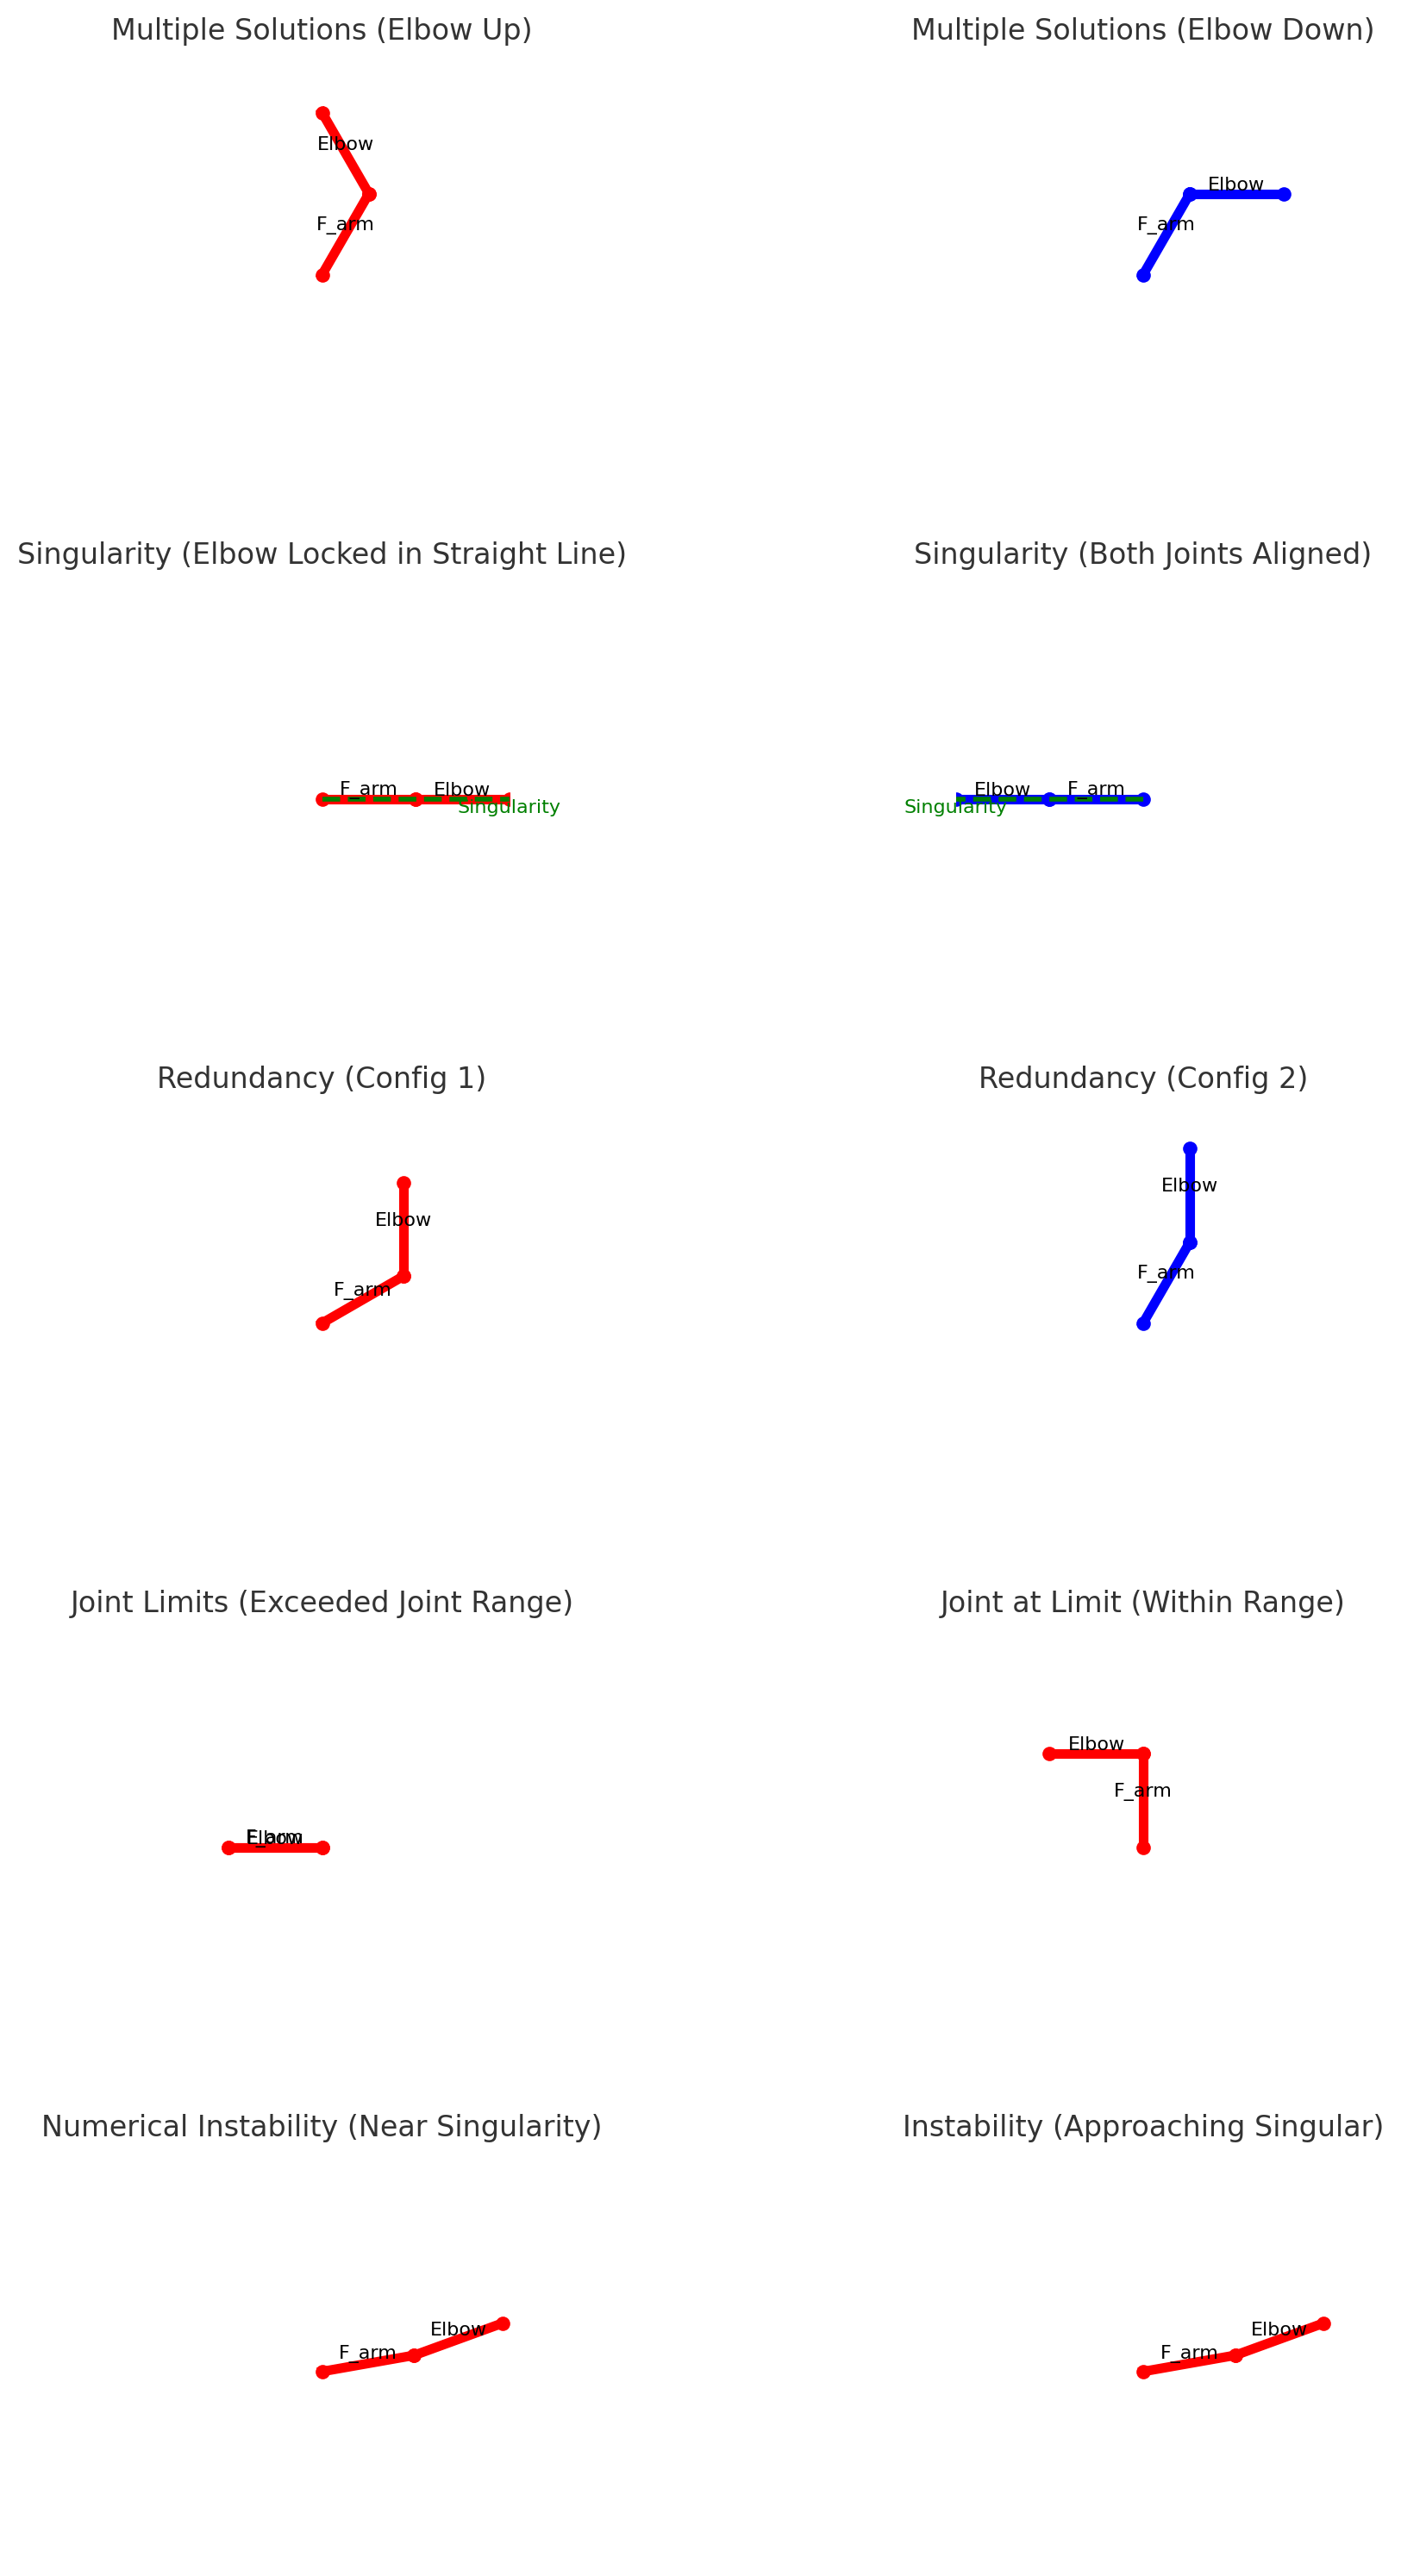
\includegraphics[width = 2.5in]{chapters/pose_matching/images/problems_classical.png}
  \caption{Problems with classical IK solving methods}
  \label{fig:problems_classical}
\end{figure}

\subsection{Data-Driven IK Approaches}
\label{subsec:data_driven_ik}

The limitations of classical IK methods have spurred the development of data-driven approaches, which leverage large datasets and machine learning to improve the realism and flexibility of character animations.

Motion Matching represents a significant shift from traditional IK by utilizing a large database of motion capture (mocap) data. Instead of predefined animation clips, Motion Matching dynamically selects the most appropriate pose based on user inputs and contextual parameters. This approach was notably employed by Ubisoft in the game For Honor, where it enabled more fluid and responsive character animations\ref{fig:for_honor}. Motion Matching's ability to break down animations into fine-grained clips allows for seamless transitions and more natural movements\cite{TODO}.

\begin{figure}
  \centering 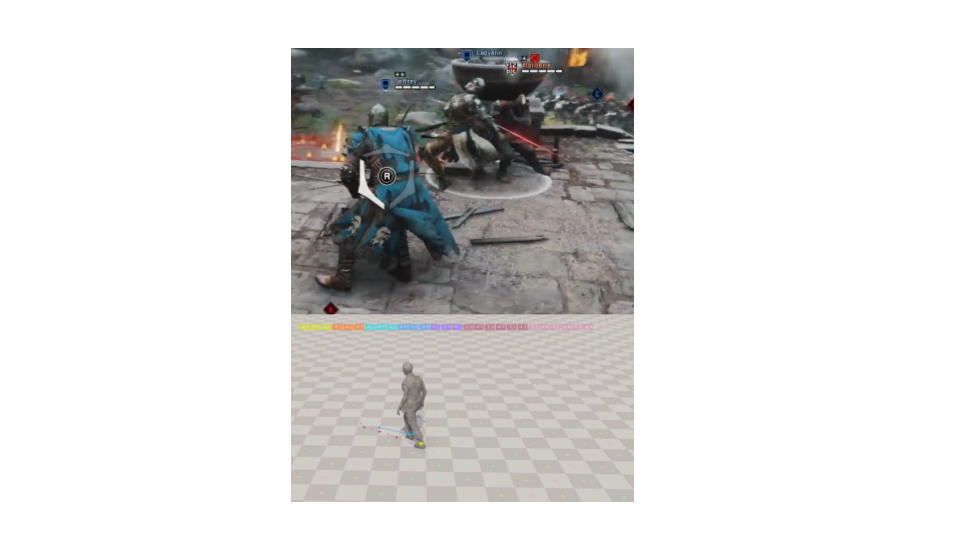
\includegraphics[width = 2.5in]{chapters/pose_matching/images/for_honor.png}
  \caption{Motion Matching in For Honor}
  \label{fig:for_honor}
\end{figure}

Phase-Functioned Neural Networks (PFNN) \cite{TODO} extends the capabilities of motion matching by incorporating phase information into the neural network's weights. This phase-aware approach allows the network to generate contextually appropriate animations that account for the cyclical nature of bipedal movement, such as walking or running. Unlike traditional methods that rely on blending animation clips, PFNN encodes the entire animation process within the neural network, offering greater flexibility and control.

\begin{figure}
  \centering 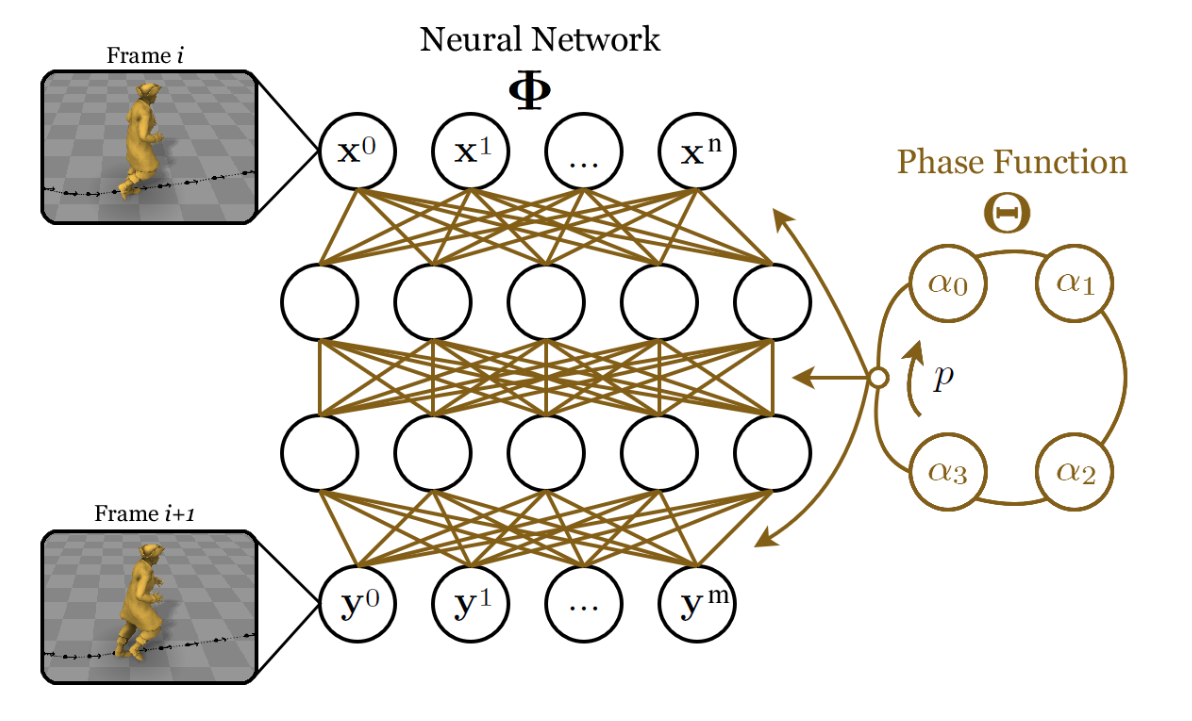
\includegraphics[width = 2.5in]{chapters/pose_matching/images/pfnn.png}
  \caption{Phase-Functioned Neural Networks (PFNN) for motion matching}
  \label{fig:pfnn}
\end{figure}

Style-Based Inverse Kinematics (Style IK) leverages machine learning to represent poses in a latent space, where the distribution of poses can be learned and sampled. Using Scaled Gaussian Process Latent Variable Models (SGPLVM), Style IK can generate stylized animations that conform to specific aesthetic or functional constraints. This approach is particularly useful for creating animations that need to adhere to a particular style or where mocap data is not available\cite{TODO}.

\begin{figure}
  \centering 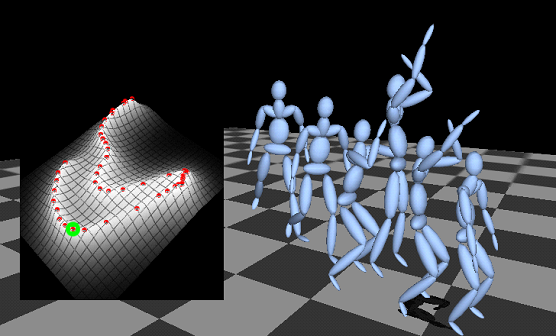
\includegraphics[width = 2.5in]{chapters/pose_matching/images/style_ik.png}
  \caption{Pose in latent space using Style IK}
  \label{fig:style_ik}
\end{figure}

These data-driven approaches represent a significant advancement over classical IK methods, offering greater flexibility, realism, and the ability to handle complex, non-linear constraints. However, they also introduce new challenges, such as the need for extensive training data and increased computational demands, particularly in real-time applications \ref{fig:problem_data_driven}.

\begin{figure}
  \centering \includegraphics[width = 2.5in]{chapters/pose_matching/images/problem_data_driven.png}
  \caption{TODO}
  \label{fig:problem_data_driven}
\end{figure}

\subsection{Latent Space Representations in Animation}

Latent space representations have become increasingly important in character animation, providing a powerful tool for managing the complexity of pose and motion data. Variational Autoencoders (VAEs)\cite{TODO}, such as the one used in SMPLify-X\cite{TODO}, learn a probabilistic model of human poses, allowing for the generation and manipulation of poses in a lower-dimensional space. In the context of pose estimation, VAEs help in predicting 3D poses from 2D images by learning a latent space that captures the distribution of plausible human poses. This latent space can then be sampled to generate realistic poses that meet specific constraints, such as end-effector positions or overall body posture\ref{fig:simplifyx}.

\begin{figure}
  \centering 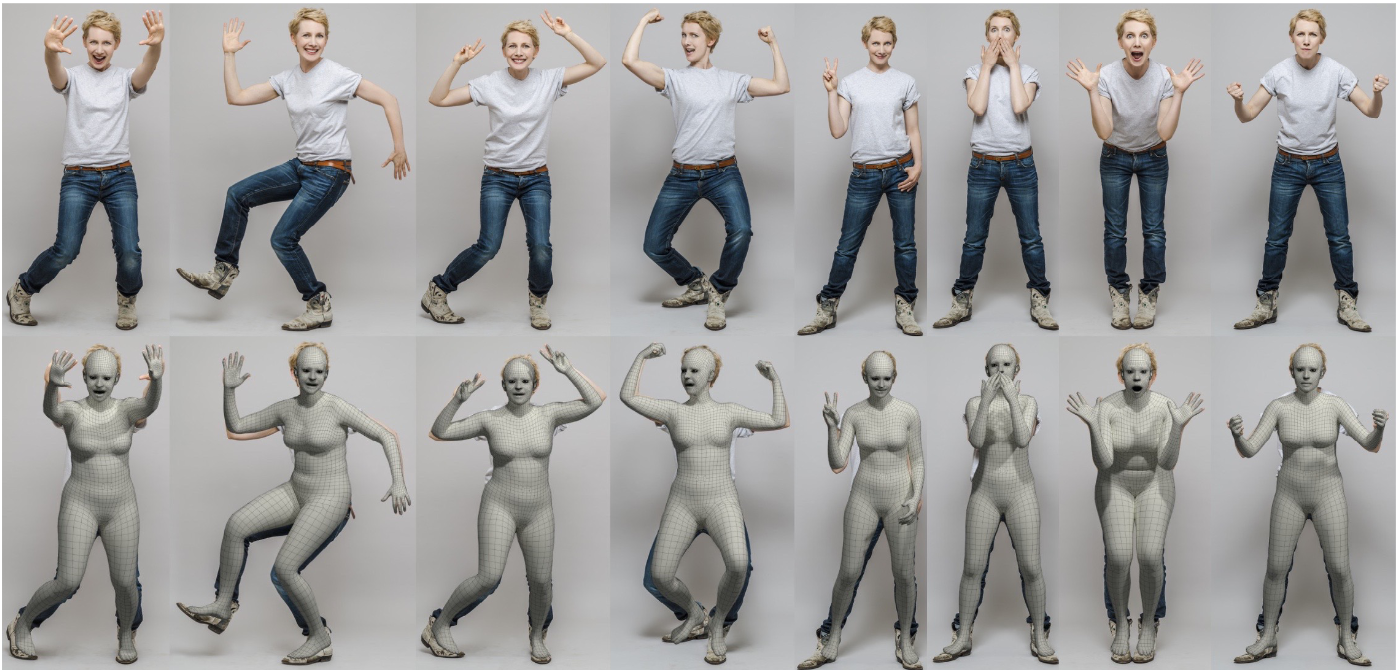
\includegraphics[width = 2.5in]{chapters/pose_matching/images/simplifyx.png}
  \caption{SMPLify-X}
  \label{fig:simplifyx}
\end{figure}

The use of latent space not only reduces the dimensionality of the data, making it easier to work with, but also enables more sophisticated manipulations, such as style transfer or the synthesis of new poses that blend characteristics from multiple examples. This has proven particularly valuable in scenarios where high-quality mocap data is not available, or where the goal is to create stylized or non-standard animations.

VPoser\cite{TODO}, a specific implementation of a VAE, further demonstrates the power of latent space in animation. By encoding poses into a low-dimensional latent space, VPoser can be used in optimization processes to ensure that generated poses are both realistic and meet specific criteria. This approach is particularly effective in applications like pose estimation from monocular images, where the latent space helps to regularize the solution and avoid physically implausible poses.

Overall, latent space representations have become a crucial component of modern character animation, enabling more complex and realistic animations while also providing tools for creative control and manipulation.

\section{Pose Matching with AZee Low Level synthesis}
\label{sec:pose_matching_with_azee}

\section{Conclusion}
\label{sec:conclusion}

The application of these advanced techniques varies significantly between real-time systems, such as video games, and production environments, such as film or high-quality CGI.

In real-time systems, the primary challenge is balancing the quality of the animation with the computational constraints of running at interactive frame rates. Techniques like Motion Matching and PFNN have been particularly successful in this domain, as they offer a good balance between realism and efficiency. However, the increased complexity of data-driven and latent space methods often requires careful optimization to meet the performance requirements of real-time systems.

In contrast, production environments can afford to prioritize the quality and stylization of animations over computational efficiency. Here, methods like Style IK and latent space models like VPoser shine, as they allow for more detailed and stylized animations that would be difficult or impossible to achieve with traditional methods. The ability to generate and manipulate animations in a latent space also offers new possibilities for creativity, enabling artists to explore a wider range of styles and movements.

Despite these advances, challenges remain in both domains. In real-time applications, the computational demands of data-driven approaches can still be prohibitive, particularly as the complexity of the animations increases. In production environments, the integration of machine learning models into existing pipelines requires careful consideration of the trade-offs between control, quality, and the effort required to train and maintain these models.

While the integration of machine learning into character animation offers numerous advantages, it also introduces new challenges.

Computational Costs: Data-driven and latent space methods typically require significant computational resources, both during training and inference. This can be a major barrier in real-time applications, where low latency is critical.

Data Availability: The effectiveness of machine learning models depends heavily on the availability of high-quality training data. In many cases, obtaining sufficient mocap data can be difficult, especially for non-standard or stylized animations.

Creative Control: While machine learning models can generate realistic and high-quality animations, they often lack the fine-grained control that human animators require. Ensuring that these models produce outputs that align with artistic vision remains a significant challenge.

In conclusion, while machine learning has opened new possibilities in character animation, it has also introduced new complexities and challenges. Future work will need to address these issues to fully realize the potential of these technologies in both real-time and production environments.

\end{document}